\documentclass[10pt,a4paper,english]{exam}
\usepackage[utf8]{inputenc}
\usepackage[T1]{fontenc}
\usepackage[english]{babel}

% Quelques paquets ...
%\usepackage{color} 
\usepackage[usenames,dvipsnames]{xcolor}
\usepackage{amsmath}
\usepackage{amssymb}
\usepackage{graphicx}
\usepackage{enumitem}
\usepackage{tcolorbox}
\usepackage{framed}
\usepackage[framemethod=tikz]{mdframed}

% Mise en page
\usepackage{geometry}
\geometry{hmargin=2.5cm,vmargin=2cm}

% Quelques commandes
\newcounter{mainmemorder}
\newcommand{\save}{\setcounter{mainmemorder}{\value{enumi}}}
\newcommand{\load}{\setcounter{enumi}{\value{mainmemorder}}}
\newcommand{\mytext}[1]{\colorbox{lightgray}{\texttt{#1}}}

% Examen
\printanswers \shadedsolutions
\noprintanswers
\newcommand{\bareme}[1]{\textbf{\newline\color{red}#1pts} -}

\global\mdfdefinestyle{graybox}{%
  linecolor=black,linewidth=1pt,%
 % leftmargin=1cm,rightmargin=1cm,%
  backgroundcolor=lightgray
}

\mdfdefinestyle{evaluation}{
    frametitlebackgroundcolor=black!15,
    frametitlerule=true,
    roundcorner=10pt,
    middlelinewidth=1pt,
    innermargin=0.5cm,
    outermargin=0.5cm,
    innerleftmargin=0.5cm,
    innerrightmargin=0.5cm,
    innertopmargin=\topskip,
    innerbottommargin=\topskip,
    frametitle={Evaluation}
}
\newcommand\blfootnote[1]{%
  \begingroup
  \renewcommand\thefootnote{}\footnote{#1}%
  \addtocounter{footnote}{-1}%
  \endgroup
}

% C'est parti .......
\begin{document}

% Titre
{\large
%\noindent NOM/Prénom :  \hspace{6cm} Num. étudiant :\\
\begin{center}
	{
		\textbf{Sorbonne Université -- Département de Sciences De l'Ingénieur\\}
		\textbf{ROS and experimental robotics}}\\
	\emph{March 2022, 1h30. \\
		%\vspace{0.4cm}
	}
\end{center}}

You are in charge of the development of a mobile robot called \texttt{mybot}, endowed with 2
directional wheels. This robot is also equipped with $12$ ultrasound sensors (US), see
Figure~\ref{fig:robot}. Each sensor of the ultrasound array aims at estimating the distance to the
obstacles around the robot through a time-of-flight computation: a short high frequency burst is
sent by the US emitter, which comes back to an US receiver when an obstacle is present. Each sensor
actually measures the time taken by the wave to go back and forth, which is a function of the speed
of sound ($c \approx$ 340 $\text{m.s}^{-1}$) and the distance $d$ to the obstacle. The US sensor
documentation indicates:
%
\begin{tcolorbox}
	\textit{Each US sensor is not able to measure any distance greater than $5m$, or smaller than $5cm$.}
\end{tcolorbox}

In practice, the ROS interface to the sensors array relies on a node
\mytext{mybot\_usarray} which communicates directly with the array of US sensors, and publishes
(among other things) an array containing the $12$ time-of-flight values (in $s$) for each US sensor
on the topic \mytext{/usarray}. In this topic, the data are arranged in the sensor IDs order, see
again Figure~\ref{fig:robot}.

Unfortunately, it appears that one or multiple US sensor(s) in the whole array might sometimes be
broken. The symptoms may vary:  sometimes the faulty sensor(s) send(s) the same value everytime
regardless of the actual obstacle distance, sometimes the sensor exposes a negative time-of-flight
or very small or large, unrealistic, value. Then, the \mytext{mybot\_usarray} node exposes a service
\mytext{/usarray\_mngt} which allows to deactivate the faulty sensor(s) in the array. The
documentation of the \mytext{mybot\_usarray} node for the service \mytext{usarray\_mngt} explains :

\begin{tcolorbox}
	\textit{The node exposes a service named \mytext{usarray\_mngt}. The message type used in the
		service is declared in the \texttt{srv} folder of its ROS package. As in input, you have to
		provide the ID of the sensor you want to activate or deactivate. You also have to provide a
		text containing either "ACTIVATE", "DEACTIVATE" or "STATUS" to use the service. When using
		"STATUS", the provided ID is not used by the service. As a response, you will get a text
		validating your request.}
\end{tcolorbox}

Your objective is to verify if you have a faulty unit in your robot US sensors array, localize it,
deactivate it, and then to write an emergency stop ROS node that should send a speed of 0 to the
\mytext{/cmd\_vel} topic used by the \mytext{mybot\_control} node to drive the robot. Your node must
also expose a service \mytext{is\_running} which should specify if you are in a state where an
emergency stop has been ordered.

\begin{mdframed}[style=evaluation]
	At the end of the exam, you have to upload two files to Moodle:
	\begin{itemize}
		\item A PDF report, written with \texttt{openoffice} for example (in french or english), where
		      you answer to the questions below and where you can copy and past the outputs of the
		      different commands you use to answer the questions. For example, for the question ``3.
		      List all the running nodes'', you must put in your report :
		      \begin{itemize}
			      \item the exact command line you use to answer the question,
			      \item and the corresponding output you get.
		      \end{itemize}
		      Obviously, you have to comment all your responses. A simple copy and past without a
		      sentence explaining the outputs is \textbf{not} considered as a full response to the
		      questions.
		\item A \texttt{zip} file of your node that will be used to access your code, but also to
		      actually launch your own package and nodes.
	\end{itemize}
\end{mdframed}

\section*{Preparation}
\begin{enumerate}
	\item To begin with, download the file \texttt{mybot.zip} from Moodle. Extract it in the
	      \texttt{src} folder of your catkin workspace. Launch \mytext{catkin\_make} to build your
	      ROS workspace and source you \texttt{.bashrc}.
	\item Go to the \texttt{src} folder of the package \mytext{mybot} you just downloaded, and make
	      executable all the python scripts in there.
	\item Quickly test that all is OK by running the node \mytext{mybot\_usarray}. Contact your
	      teacher if it is not the case.
	      \save
\end{enumerate}


%===================================================================================================
\section{Exploration of ROS and of the nodes}

\begin{enumerate}
	\load
	\item Run the nodes \mytext{mybot\_usarray} and \mytext{mybot\_control} from the package
	      \mytext{mybot}. Then list all the running nodes.

	      \begin{solution}
		      \begin{verbatim}
> rosnode list
/mybot_control
/mybot_usarray
/rosout	      			
		\end{verbatim}
		      3 nœuds tournent : les 2 nœuds attendus et \mytext{rosout}, lancé avec le master via la
		      commande \texttt{roscore}.
	      \end{solution}
	\item List the information about the \mytext{mybot\_usarray} node. Explain each line of the output
	      you get.

	      \begin{solution}
		      \begin{verbatim}
> rosnode info /mybot_usarray
--------------------------------------------------------------------------------
Node [/mybot_usarray]
Publications:
 * /rosout [rosgraph_msgs/Log]
 * /usarray [std_msgs/Float64MultiArray]

Subscriptions: None

Services:
 * /mybot_usarray/get_loggers
 * /mybot_usarray/set_logger_level
 * /usarray_mngt


contacting node http://127.0.0.1:54662/ ...
Pid: 24039
Connections:
 * topic: /rosout
    * to: /rosout
    * direction: outbound (54664 - 127.0.0.1:54667) [10]
    * transport: TCPROS			\end{verbatim}
		      Je ne vais pas tout lister (mais les étudiants doivent le faire !). La dernière partie
		      n'est souvent pas comprise :
		      \begin{itemize}
			      \item \verb+contacting node http://127.0.0.1:56353/ ...+: adresse et port où
			            tourne le nœud
			      \item \verb+Pid: 12097+: Process Identification du numéro du processus
			      \item  \verb+* direction: outbound (56355 - 127.0.0.1:56358) [10]+: type de
			            connexion, et vers quelle addresse/port (ici, celui du master)
			      \item \verb+* transport: TCPROS+: protocole utilisé par ROS, ici une connection
			            TCPROS.
		      \end{itemize}
	      \end{solution}
	\item List all the available topics. Explain the role of the \mytext{/rosout} topic.
	      \begin{solution}
		      \begin{verbatim}
> rostopic list
/cmd_vel
/rosout
/rosout_agg
/usarray	
			   \end{verbatim}
		      \texttt{/rosout} is le topic sur lequel les nœuds peuvent publier des messages de log de manière
		      centralisée.
	      \end{solution}

	\item What kind of message is available on the \mytext{/usarray} topic? Detail each field of the
	      message.
	      \begin{solution}
		      \begin{verbatim}
> rosmsg info std_msgs/Float64MultiArray
std_msgs/MultiArrayLayout layout
  std_msgs/MultiArrayDimension[] dim
    string label
    uint32 size
    uint32 stride
  uint32 data_offset
float64[] data
		\end{verbatim}
		      Structure qui présente l'organisation des données (nom, dimension, etc.) + une array data qui stocke
		      les valeurs.
	      \end{solution}
	\item Display a few messages available on the topic \mytext{/usarray}. At which rate are they
	      published?
	      \begin{solution}
		      \begin{verbatim}
> rostopic echo /usarray
layout:
  dim:
    -
      label: "times of flight"
      size: 12
      stride: 1
  data_offset: 0
data: [0.01878487746072629, 0.018874952200062568, 0.019142913108409175, 0.00590796102128278, 0.0057507262774564825, 0.004326279897161326, 0.004007958769269939, 0.004079208299596867, 0.004105389496859937, 0.012378029560149738, 0.012074491972118843, 0.011963473874609925]---
---
layout:
  dim:
    -
      label: "times of flight"
      size: 12
      stride: 1
  data_offset: 0
data: [0.018748515836326585, 0.018441489413458696, 0.018488714226558824, 0.0059762322824051285, 0.005831043094898178, 0.004326279897161326, 0.004087100107586651, 0.004155806903870856, 0.00404233845708314, 0.012122213535348885, 0.01204055757308907, 0.012072762095295621]

> rostopic hz /robot_sensor
subscribed to [/usarray]
no new messages
average rate: 0.799
	min: 1.251s max: 1.251s std dev: 0.00000s window: 2
average rate: 0.800
	min: 1.250s max: 1.251s std dev: 0.00025s window: 3\end{verbatim}
		      Publication à 0.8Hz environ.
	      \end{solution}
	      \save
\end{enumerate}

%===================================================================================================
\section{Emergency stop node}

You have to write a new ROS node \mytext{emergency\_stop} which should trigger an emergency stop
when the robot detects an obstacle \textbf{in front or behind it}. This emergency stop must be
activated by publishing a null speed to the \mytext{/cmd\_vel} topic of the \mytext{mybot\_control}
node  as soon as the distance $d$ to the obstacle detected \textbf{by any sensor in the front or
	back of the robot} is smaller than a threshold (expressed in meters) than can be tuned manually. If
no obstacle is detected, then the robot is expected to go straight at a speed of your choice.
\begin{enumerate}
	\load
	\item Create a package \mytext{exam} with dependencies to \texttt{rospy}, \texttt{std\_msgs} and \texttt{mybot} ;
	      \begin{solution}
		      catkin\_create\_pkg exam rospy std\_msgs mybot
	      \end{solution}
	\item Create the node \mytext{emergency\_stop} which should subscribe and publish to the
	      adequate topics by using \texttt{rospy}:
	      \begin{enumerate}
		      \item Define a variable \texttt{threshold} in your code that can be used to tune the
		            obstacle detection. By default, an obstacle closer to $0.5m$ must trigger an emergency
		            stop ;
		      \item Print a message "\texttt{GO}" or "\texttt{STOP}" in the terminal and publish a
		            null speed with the \textbf{first detection only} of presence of an
		            obstacle.
		      \item Create a launch file where the three nodes \mytext{mybot\_control},
		            \mytext{mybot\_usarray} and \mytext{emergency\_stop} are launched together, and
		            where the distance threshold is set ;
		      \item Create a ROS parameter \texttt{threshold} in your launch file that you can use
		            to define the above \texttt{threshold} variable in your code.

	      \end{enumerate}
	      \save
\end{enumerate}

\begin{mdframed}[style=evaluation]
	It is important you comment extensively your code, even for elementary lines of code. Your node
	will be assessed by running your node (it must obviously run as expected and provide the
	functionalities listed above), but the quality of the code and its comments will also be taken
	into account.
\end{mdframed}

\begin{enumerate}
	\load
	\item Using the service \mytext{usarray\_mngt}:
	      \begin{enumerate}
		      \item Inspect the output of your node. Knowing that your robot is inside an empty
		            rectangular room, does it work as expected?
		      \item Inspect carefully the message sent by the US sensors. What can you see? Propose
		            a solution using the \mytext{usarray\_mngt} service.
	      \end{enumerate}
	\item Publication of the distance information:
	      \begin{enumerate}
		      \item Modify your node so that it now publishes to a new topic \mytext{/distance} the
		            four mean\footnote{To that end, you might be interested in the function
			            \texttt{nanmean()} from \texttt{numpy}.} \textbf{distances} (corresponding to the
		            four directions) to the obstacles around the robot.
		      \item On the basis on the output of the \mytext{/distance} topic, place the walls
		            around the robot in Figure~\ref{fig:robot} (do not forget to specify the scale on your
		            plot!)
	      \end{enumerate}
	\item (Bonus) Creation of the service \mytext{is\_running}:
	      \begin{enumerate}
		      \item Create a service named \mytext{is\_running}, expecting a message of type
		            \texttt{std\_srvs/Trigger} and returning a string "\texttt{GO}" or "\texttt{STOP}"
		            depending on the state of the emergency stop.
		      \item Test you service with the command \texttt{rosservice}.
	      \end{enumerate}

\end{enumerate}

\newpage

\begin{figure}
	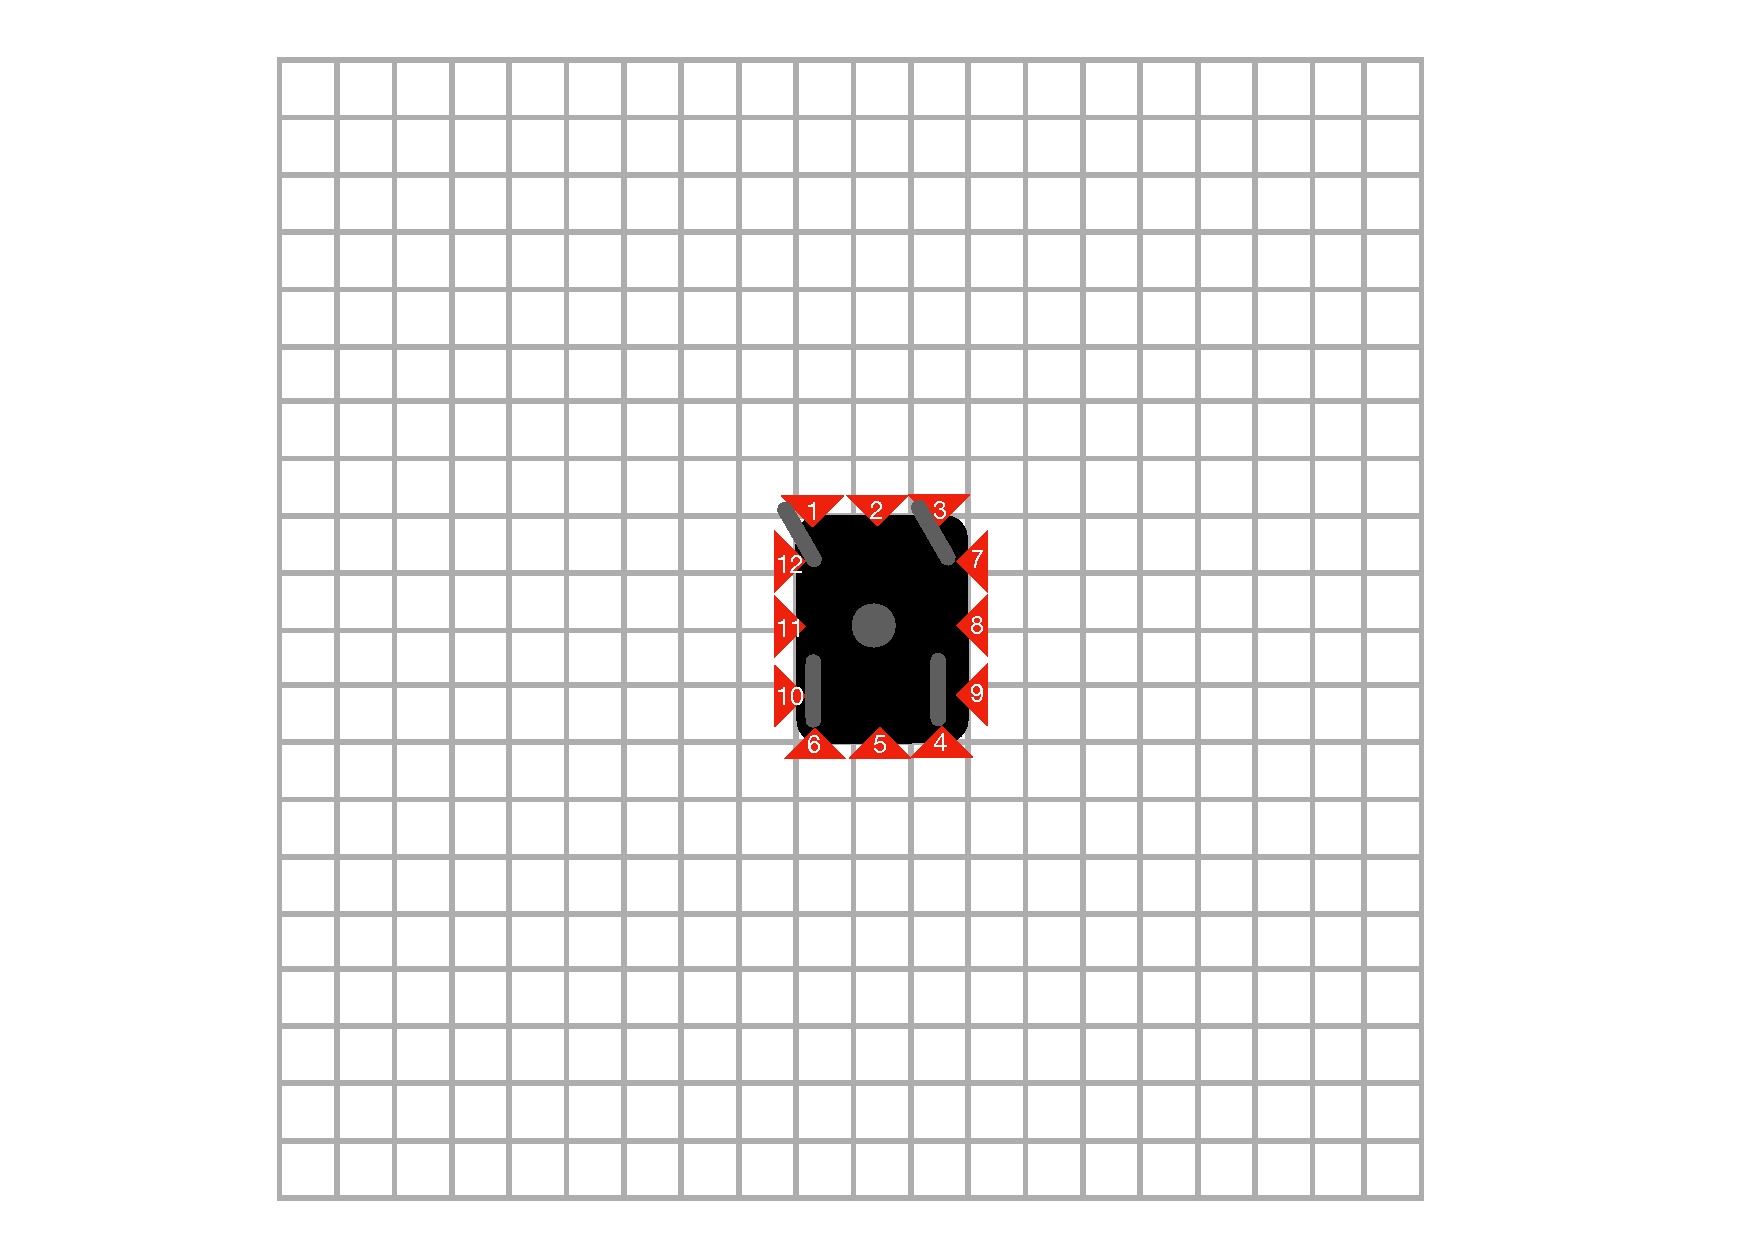
\includegraphics[width=\linewidth]{images/robot.pdf}
	\caption{View of the \texttt{mybot} robot and of its US sensors (in red) spatial organization.
		Each sensor is identified with an \texttt{ID} number (in white) inside the sensor array.}
	\label{fig:robot}
\end{figure}

\end{document}
